\section{IoTサービスの構造と事例}
IoTとは、「モノのインターネット」とも呼ばれる、様々なモノがインターネットを介して通信し合うことで自動化を図る概念である。
IoTサービスとは、IoTによる利便性を顧客へ提供するものである。

IoTサービスは、図のようにIoT機器、ネットワーク(インターネット)、サーバから構成されている。
\begin{figure}[htbp]
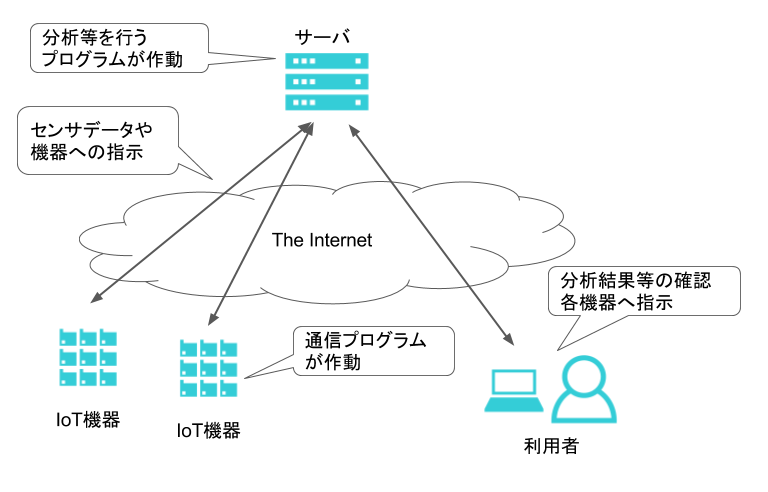
\includegraphics[width=16cm]{images/IoTstract.png}
\caption{IoTサービスの構造図}
\label{fig:iotstract}
\end{figure}

IoT機器は、RaspberryPiやEdison等の小型コンピュータや組み込み機器が使用され、周辺環境を検知する他、周辺環境へ働きかける事を行う。
IoT機器では、通信プログラムが作動しており、インターネットを介して、検知した周辺環境に関する情報や、IoT機器への指示をやり取りする。
IoT機器は、Wifiや有線接続等を用いて、インターネットへ接続された携帯電話網や社内LAN等のネットワークに接続される。

サーバは、インターネット上に設置され、蓄積・分析・可視化等を行うプログラムが作動している。
このプログラムは、IoT機器から送られてきた情報を蓄積・分析し、必要に応じてIoT機器へ指示を送る他、分析結果を利用者へ可視化する。

利用者は、サーバへインターネットを介して接続し、分析結果の閲覧・機器への指示を行う。

\section{IoTサービス開発の事例}

\subsection{株式会社ルナネクサスでの事例}
株式会社ルナネクサスでは、太陽光発電事業を展開している事業主に対し、発電に係る機器の状態や、発電量等を可視化できるサービスを展開している。
太陽光発電は、太陽光パネルと発電した電力を送電する為の「パワーコンディショナ」と呼ばれる機器で成り立っている。
株式会社ルナネクサスでは、そのパワーコンディショナに独自に開発したIoT機器を取り付け、発電量や発電機器の異常などを収集する。
収集したデータは、SORACOM Airという携帯電話網を利用したインターネット接続サービスを使用してインターネット上にあるサーバへ送信される。
サーバ上では、各IoT機器から送られてきた情報を蓄積し、可視化する。
これによって、発電事業を展開している事業主に、各発電所まで行かなくても発電量や発電機器の異常等を確認することができる、という利便性を提供している。
図\ref{fig:lunafig}は株式会社ルナネクサスのIoTサービスイメージである。
\begin{figure}[htbp]
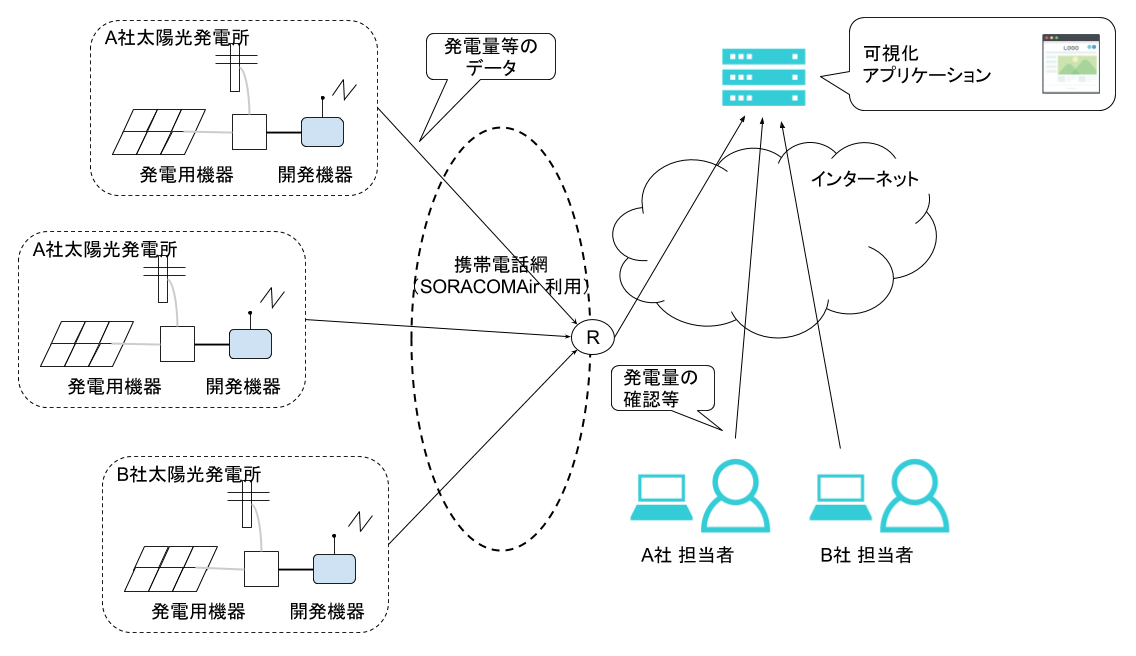
\includegraphics[width=16cm]{images/lunafig.png}
\caption{株式会社ルナネクサス サービスイメージ図}
\label{fig:lunafig}
\end{figure}
太陽光発電所は僻地にあることが多いので、利用できるネットワークが無いことが多い。
このことから、インターネットへの接続にSORACOM Airを選択した。

しかし、SORACOM Air回線は、プライベートアドレスを使用しており、IoT機器からの通信は通過するものの、インターネット側からPingなどによる確認を行うことが出来ない。
そのため、各IoT機器の監視とメンテナンスの為に、VPNを利用し、定期的にVPN越しにログインすることで監視を行っている。
VPN越しにログインするためには、各IoT機器にVPNクライアントを導入し、新たにVPNサーバをたち上げる必要があった。
また、手動で各機器へログインすることは、手間である。

\subsection{岡本商店街における事例}
岡本商店街とは、神戸市東灘区にある阪急岡本駅とJR摂津本山駅の間にある商店街のことで、
商店街の方に人流を可視化するIoTサービスを提供し商店街の活性化に役立てるといった趣旨で、2016年2月7日から2016年3月14日まで観測を行った。
人流観測とは、各地点から各地点迄をある時に移動した人数を観測するものである。
今回は、ある地点を通過した人物が以前どの地点を通過していたのかを観測したかった為、携帯電話についているWifi機能が送出する電波を利用して観測を行うこととした。
観測・分析・可視化を行うシステムの構成としては図\ref{fig:okamoto_diag1}の様になる。
各店舗に設置させてもらった観測機器は、店舗に敷設されたネットワーク回線を通して、インターネットへと繋がっている。
各観測機器は、観測したデータをインターネット上のサーバへと送信し、そのサーバの上で蓄積・分析・可視化を行う形となっている。
\medskip

\begin{figure}[htb]
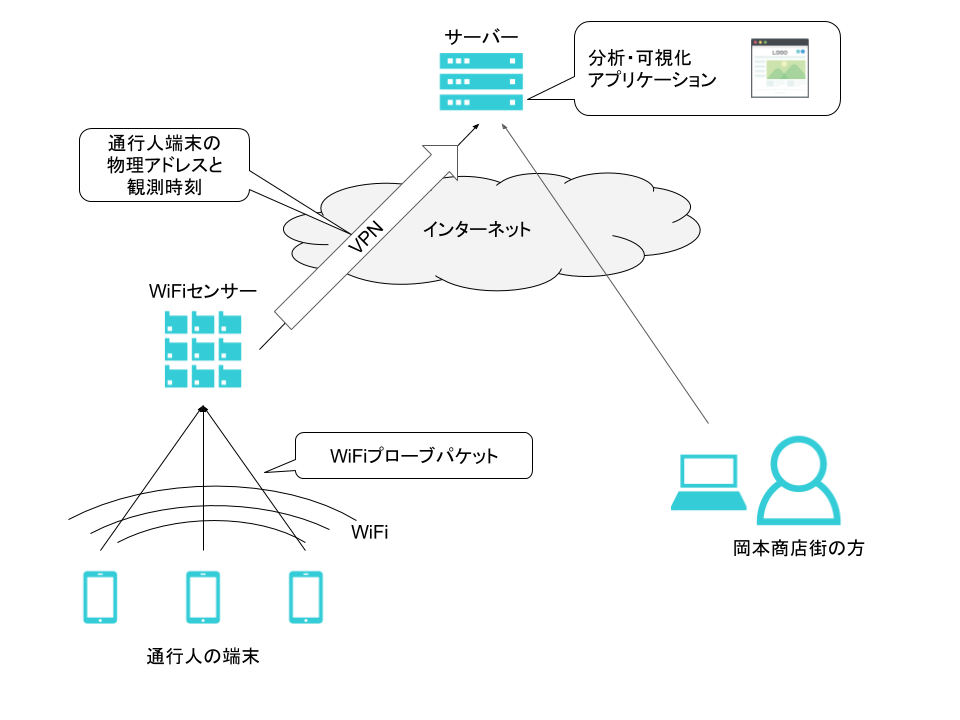
\includegraphics[width=16cm]{images/okamoto_diag1.png}
\caption{岡本商店街人流観測 構成図}
\label{fig:okamoto_diag1}
\end{figure}

実験の際に、次の様な問題や負担があった。
\begin{itemize}
\item 電源が抜けている・ネットワークが切断されているといった要因で、観測できていないことがあった。
\item 上記要因にて観測できていない事に気づくことが遅れた。
\end{itemize}
これらから、IoT機器の監視が必要と考え、VPN越しにログインすることで、確認を行うこととした。
しかし、各観測機器にVPNを介してログインすることは手間であり、負担であった。
また、実験では観測機器の数が5台のみであったが、大規模に観測を行うことを考えた場合、手動での確認はとても大きな負担となる。
そのため、効率化を図る必要があったと感じる。

\section{IoTサービスの提供者の課題}
これら事例と実験からIoTサービスの円滑な提供において、開発は容易だが、IoTサービスの構造を維持するために、IoT機器の監視・管理が必要となっている事が分かった。
しかし、IoT機器の監視・管理には、次のような課題がある。
\begin{itemize}
\item IoT機器が多量である\\
	そのため、各機器へ設定することは大きな負担となる。
	また、監視サーバへの登録も負担となる。
\item IoT機器が接続されるネットワークが多様である\\
	そのため、既存の問い合わせによる監視手法は適応できない。
	しかし、通知による監視を行うには、各機器へ設定する必要がある。
\item IoT機器の追加や交換が頻繁にある\\
	そのため、監視サーバへの登録作業を頻繁に行う必要がある。
\item 外観が似通っている\\
	そのため、交換のため現地に行くも、交換すべき機器がどれなのか判別がつかない。
\end{itemize}

私は、その中でも、監視サーバへの登録の負担とIoT機器への設定の負担について取り上げ分析することにした。
IoT機器の監視のためには、IoT機器が接続されるネットワークの多様性から、IoT機器からの通知による監視手法を取らざる終えない。
しかし、そのためにはIoT機器と監視サーバに対し、識別子(ID)を設定する必要がある。
IoT機器に対し、固有の識別子を与え、監視サーバに識別子を伝えることで、監視サーバはどの機器からの通信なのか見分けることができる。
また、監視サーバに対し、予め識別子を設定しておくことで、監視対象とする機器以外からの不正なアクセスを遮断することができる。
よって、IoT機器へ識別子を設定し、監視サーバに対して登録を行う必要がある。
しかし、IoTサービスでは、IoT機器が多量に使用されることや、頻繁な交換・追加・撤去がありうるため、
これら設定や、設定の変更は大きな負担となっている。


\begin{comment}
前項で述べたとおり、株式会社ルナネクサスでは、各IoT機器のメンテナンスと状態の確認の為に、VPNを利用して遠隔から手動でログインすることを行っている。
各機器のメンテナンスは頻繁には行っていないが、各IoT機器の稼働の確認は定期的に行っている。
現在、IoT機器は十数台しかないが、今後、増えていく事が予想されるため、各IoT機器の稼働の確認が大きな負担となる。

この問題について調べる為に、株式会社ルナネクサスへインタビューを行ったところ、次のような要望があった。
\begin{itemize}
\item 単純に機器が起動し、動作している事が確認できれば良い
\item 欲を言うと、CPUの温度等も確認できれば良い
\item 各機器に対するVPNや監視の為の設定も簡略化できたら尚良い
\end{itemize}
\end{comment}

